\chapter{User Guide}\label{appendix:user_guide}
This Appendix contains notes for installing and running the simulation. A copy of the code was submitted with this report. The latest version of the code can be found on Github at \url{https://github.com/henryaddison/siver}.

There are two options for running the simulation. One of Repast's nice features is it provides a way of bundling up the code into a single jar which can then be run by anyone simply by double clicking. Such an executable was submitted on CATE along with the source code. The other alternative is to compile and run the code from source. In BOTH cases, MySQL will need to be installed first and the database created with the correct schema.

\section{Setting up MySQL database}

\subsection{Installing MySQL}

Users are directed to the MySQL website, \url{http://www.mysql.com/}, for instructions on how to install MySQL. The code expects the MySQL server to be accessible on localhost.

\subsection{Creating the databases}

Next the databases used by the code need to be setup on the server. I chose to use databases called \texttt{siver\_development} and \texttt{siver\_production} to separate where data gets recorded as I worked on the code and when I was running proper experiments. The code will check an environment variable called DB\_ENV when it runs in order to determine the suffix to \texttt{siver\_}. The default database is \texttt{siver\_development} is DB\_ENV is not specified. The following SQL queries will create this database:

\begin{lstlisting}[language=SQL]
  CREATE DATABASE siver_development;
  GRANT ALL PRIVILEGES ON siver_development.* TO siver@localhost;
\end{lstlisting}

\subsection{Filling the databases}

The database schema also needs to be setup. This can be done in three ways:
\begin{itemize}
  \item load one of the full database dumps in from the /db/dumps directory in the project code.
  \item load one of the schema dumps in from the /db/dumps directory in the project code.
  \item run each of the migration SQL scripts in order in the /db/migrations directory.
\end{itemize}
For new users, I recommend the first suggestion as this will create some schedules that can be played with straight out of the box. However, new schedules can be created by the user.

\subsection{Creating schedules and simulation parameters}

% In the /db/schedule_generation directory there are a couple of ruby scripts: \texttt{create\_schedule.rb} and \texttt{create\_simulation\_parameters.rb}. Both these scripts respond to the DB\_ENV environment variable to select the database as described above and default to using the \texttt{siver\_development} database.

\subsubsection{create\_schedule.rb}

\texttt{create\_schedule.rb} will create entries in the \texttt{schedules} and \texttt{scheduled\_launches} tables corresponding the options provided. Below is the output of the \texttt{--help} option:

\begin{lstlisting}[basicstyle=\ttfamily]
Usage: create_schedule [options]
    -s, --schedule-name SNAME        Schedule name
    -v SCHEDULE_VERSION,             Schedule version
        --schedule-version
    -b, --boat-count BOAT_COUNT      Boat count
    -d, --launch-delay LAUNCH_DELAY  Launch delay
    -h, --help                       Show this message
\end{lstlisting}

Example usage: \texttt{DB\_ENV=development ruby create\_schedule.rb -s ``10 boats 1 minute delay'' -v 2 -b 10 -d 60} \\
This will create a schedule called ``10 boats 1 minute delay'' with version number 2. This schedule will have 10 boat launches scheduled and the launches will be 60 ticks apart.

\begin{description}
\item -s, --schedule-name and -v, --schedule-version\\
  Schedule name and version allow several versions of the same schedule - e.g. 5 versions of a schedule launching 10 boats with a 60 tick delay between each launch might all have name ``10 boats 1 minute delay'' but will each have a unique version number.

\item -b, --boat-count\\
  Boat count is the number of scheduled launches to create.
  
\item -d, --launch-delay\\  
  Launch delay is the number of ticks to put between each launch.
\end{description}
The desired gear for each launch is picked at random from 1 to 10. The distance to cover is fixed at 5000 and the speed multiplier for each boat is fixed at 0.5.

\subsubsection{create\_simulation\_parameters.rb}

\texttt{create\_simulation\_parameters.rb} will create entries in the \texttt{simulation\_parameters} table corresponding the options provided. Below is the output of the \texttt{--help} option:

\begin{lstlisting}[basicstyle=\ttfamily]
Usage: create_simulation_parameters [options]
    -s                               Schedule IDs
        --all-schedules
    -r, --random-seed RSEED          Random seed
    -c CONTROL_POLICY_TYPES,         List of control policy class names
        --control-policies
    -h, --help                       Show this message
\end{lstlisting}

Example usage: \texttt{DB\_ENV=development ruby create\_simulation\_parameters.rb --all-schedules -c GearFocussed,SafetyFocussed} \\
This will create two simulation parameters for for each of the schedules in the \texttt{schedules} table - one where the control policy is GearFocussed and the second where the control policy is SafetyFocussed. A constant, randomly chosen random seed will be used for all these simulation parameters.

\begin{description}
\item -s\\
  Schedule Ids to create simulation parameters entries for can be listed comma separated

\item --all-schedules\\
  Overrides the schedule ids specified by -s to use all the 

\item -r, --random-seed\\
  Specify the Random Seed associated with the simulation parameters entries being created. Default is a random number.
  
\item   -c, --control-policies\\
  Use with a comma-separated list of policy class names to create simulation parameters entries for each of the polices
\end{description}

\section{Running code from source}

\begin{enumerate}
\item Install Repast Simphony - \url{http://repast.sourceforge.net/} for instructions.

\item Run the Repast Simphony version of Eclipse just set up and import the code.

\item Eclipse will hopefully compile the code now. If it can't it may be that the required libraries and frameworks are not on the project's class path. Check that the Repast libraries are there and the JDBC MySQL driver are part of the project's build path. For simplicity I've included a copy of the MySQL driver in the lib directory. 

The lib directory also contains the dependencies for EasyMock. These are needed for the tests. If you want to run the tests then also make sure these jars.

\item The launchers directory contains launchers that Eclipse understands. These should already be set up so that all the required libraries are added to the class path. If so the code should just run. If it doesn't, check the run path in the launcher to make sure the libraries are on it as with the previous step.
\end{enumerate}

\section{Running the code from the pre-compiled jar}
Fingers crossed with the MySQL database setup this will just run.

\section{Using the simulation}
Let's imagine now you've got the application running. It should look something like Figure \ref{userguide:openingscreen}.  To the right is a window labelled Simulation Option Windows. There are 4 windows with a selector at the bottom. The Repast website (\url{http://repast.sourceforge.net/}) has more detail about these so I will cover what is particularly useful to running the simulation. 

\begin{figure}
\begin{center}
  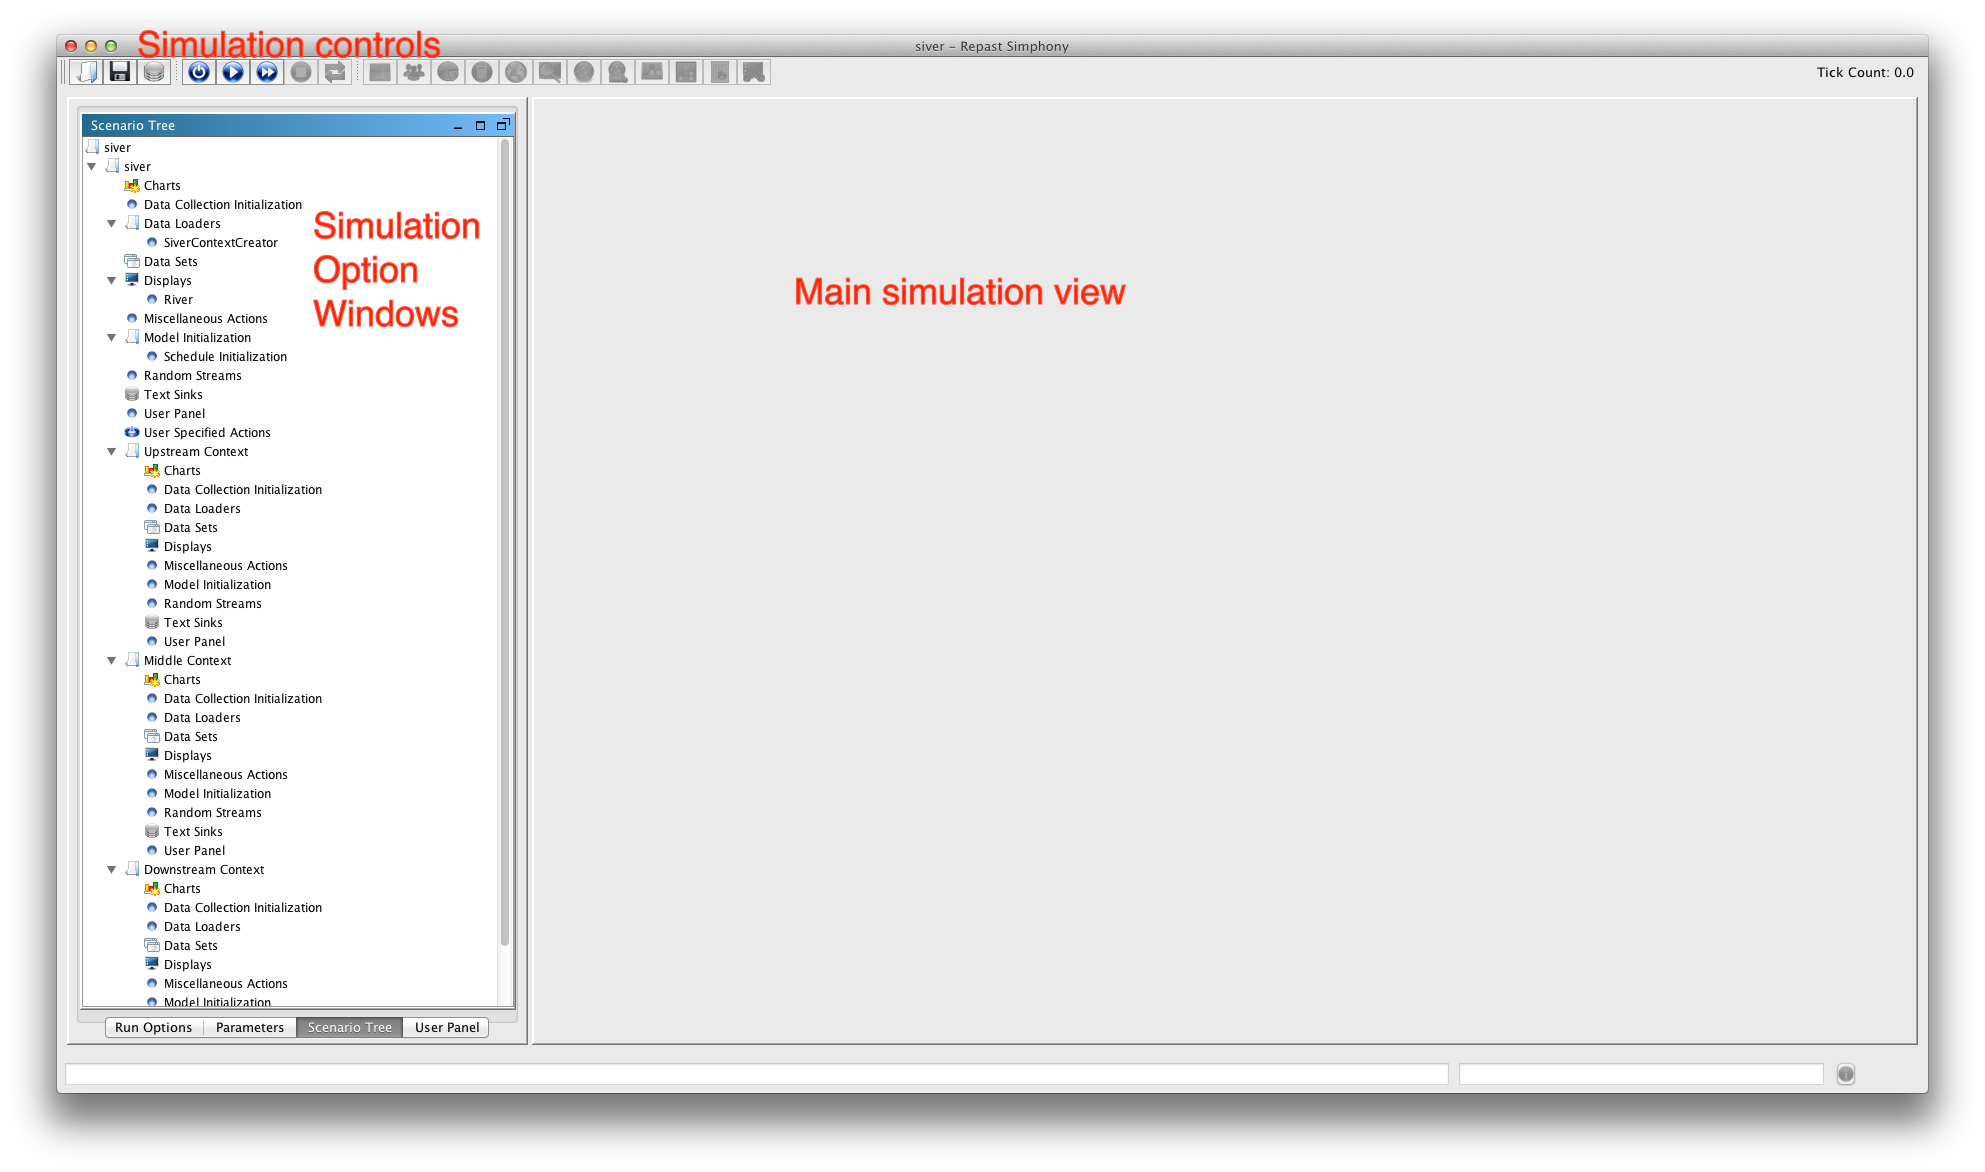
\includegraphics[scale=0.2]{images/screenshots/openingscreen.png}
  \caption{}
  \label{userguide:openingscreen}
\end{center}
\end{figure}

In this opening shot the Scenario Tree window is open. This is a GUI for setting configuration details  like how agents should be displayed and which projections should be shown in the Main Simulation View. Making changes here will alter the XML config files in the siver.rs directory.

The Parameters window, Figure \ref{userguide:parameters}, contains a field for setting the Simulation Parameter Id. If left at 0, then the simulation will run in interactive mode where the user gets to choose which boats are launched. Otherwise the simulation will look up row in the simulation\_parameters table and use those settings to determine when and what boats are launched.

\begin{figure}
\begin{center}
  \subfigure[Parameters window]{\label{userguide:parameters}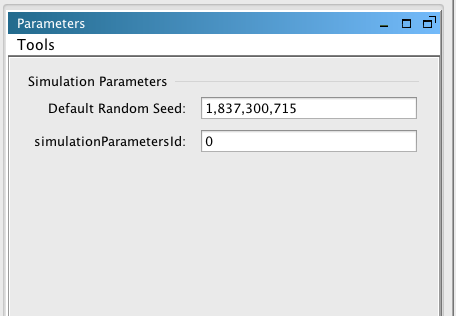
\includegraphics[scale=0.5]{images/screenshots/parameters.png}}
  \subfigure[Run Options window]{\label{userguide:runoptions}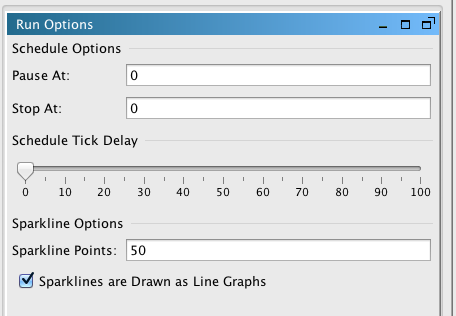
\includegraphics[scale=0.5]{images/screenshots/runoptions.png}}
  \subfigure[Simulation Control Buttons]{\label{userguide:controls} 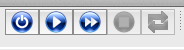
\includegraphics[scale=0.7]{images/screenshots/simulationcontrols.png}}
\end{center}
\end{figure}

The Run Options window, Figure \ref{userguide:runoptions}, can be used to put a delay between each tick using the slide labelled Schedule Tick Delay. This will slow down the simulation. When running with 0 delay, the simulation is too fast to watch. Increasing the delay will make the visualization easier to watch.


Along the top are some buttons. Of particular interest are the simulation controls just under the label that can bee seen in close up in \ref{userguide:controls}. The first button on the right will initialize the simulation. This is the point at which the Simulation Parameters Id is read. In the Main Simulation View the outline of the river should appear as in Figure \ref{userguide:interactivemodeinitialized}. The next button, the play button, will start the simulation (so the tick counter in the top right will start to increase). The pause button and stop button do the obvious of pausing and stopping the simulation. The final reset button on the left of this set will clear out the simulation so a new one can be initialized.

\begin{figure}
\begin{center}
  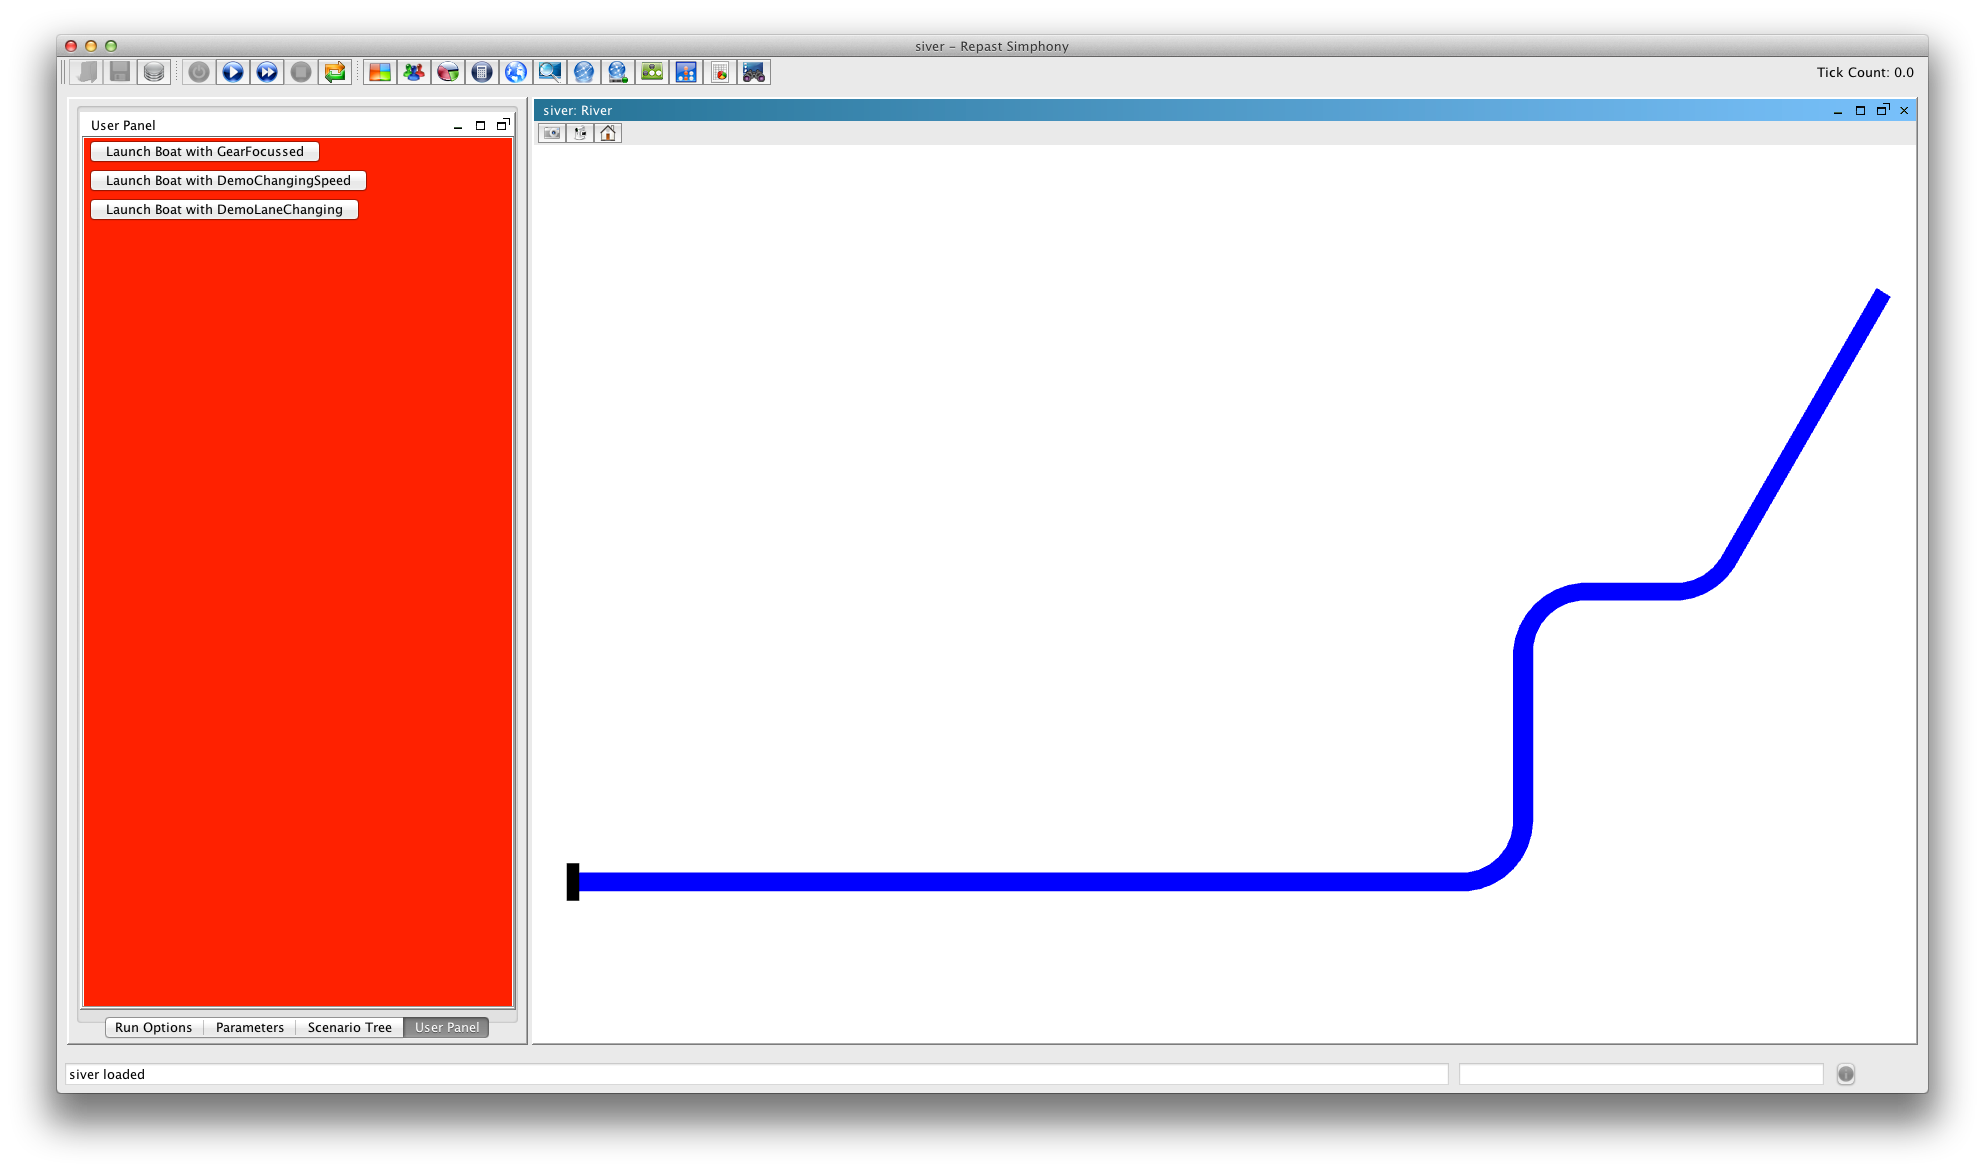
\includegraphics[scale=0.2]{images/screenshots/interactivemodeinitialized.png}
  \caption{}
  \label{userguide:interactivemodeinitialized}
\end{center}
\end{figure}

Figure \ref{userguide:interactivemodeinitialized} also shows the User Panel window. This is only active when the Simulation Parameter Id being used is 0. There are three buttons which will each cause a boat with a different control policy to be launched. The control policies available here are designed to demo the actions rather than show any intelligence.

If the simulation is not working for you then try contacting me through the Github page. The Repast mailing list may also be able to help if it's a Repast specific problem.